% Cyrinx 2.0 follow-on whitepaper.
% Build: pdflatex cyrinx-2-goodput.tex (run twice for cross-references).
% This is a separate companion to cyrinx-acoustic-link.tex, not a replacement.
\documentclass[11pt]{article}

\usepackage[letterpaper,margin=0.9in]{geometry}
\usepackage[T1]{fontenc}
\usepackage{lmodern}
\usepackage[utf8]{inputenc}
\usepackage{microtype}
\usepackage{booktabs}
\usepackage{longtable}
\usepackage{array}
\usepackage{amsmath}
\usepackage{graphicx}
\usepackage{xcolor}
\usepackage{caption}
\usepackage{url}
\usepackage[hidelinks]{hyperref}

\hypersetup{
  pdftitle={Cyrinx 2.0: Measured 65.9 kb/s Schedule-Comparable Acoustic Goodput},
  pdfauthor={David E. Weekly},
  pdfsubject={Measured MacBook Pro to Pixel 7a near-field acoustic goodput},
  pdfkeywords={acoustic modem, OFDM, goodput, microphone diversity, MRC, Cyrinx}
}

\urlstyle{same}
\captionsetup{font=small,labelfont=bf}
\setlength{\emergencystretch}{2em}
\newcommand{\kbps}{\,\mathrm{kb/s}}
\newcommand{\cyrtwo}{Cyrinx~2.0}
\newcommand{\cyrone}{Cyrinx~1.0}
\newcommand{\hash}[2]{\texttt{#1}\allowbreak\texttt{#2}}

\title{\textbf{Cyrinx 2.0: Measured 65.9\,kb/s Schedule-Comparable
Acoustic Goodput on a MacBook Pro--Pixel 7a Near-Field Link}\\[0.45em]
\large Pilot-local reliability weighting and payload-independent microphone
diversity}

\author{David E. Weekly\thanks{Primatech Paper Co LLC,
\texttt{david@weekly.org}. This report describes an open-source research
prototype developed by AI coding agents under human direction. The author
provided the physical test bench, operating constraints, and measurement
approvals.}}

\date{July 17, 2026}

\begin{document}
\maketitle

\begin{abstract}
We report \cyrtwo, a follow-on evaluation of the MacBook Pro-to-Pixel 7a
acoustic downlink. In a prospective, order-balanced eight-pair campaign that
retained the prior 48\,kHz, five-frame schedule with four 250\,ms interframe
gaps, a
CP96, pilot-spacing-16, 64-QAM rate-2/3 profile achieved
\textbf{65.875\,kb/s} mean strict ordered byte-verified scheduled goodput
(65.266--66.641\,kb/s; 4,215/4,280 blocks). The receiver used two-channel
Android \texttt{UNPROCESSED} capture, held-out-pilot selection between the
bottom microphone and two-microphone maximal-ratio combining (MRC), and
frequency-local known-pilot reliability. Its paired CP240,
pilot-spacing-8, 16-QAM rate-3/4 control achieved 44.199\,kb/s and recovered
2,999/3,000 blocks. All 16 runs completed and the candidate won all eight
pairs (exact one-sided sign test, $p=1/256$).

The result is 49.0\% above the prospective paired control and 1.801$\times$
the historical 36.571\,kb/s website target. The latter retained the same
schedule class but used expected-set membership rather than strict ordered
slot attribution. The new candidate failed its predeclared
baseline-equivalent reliability gate: 98.481\% block recovery versus
99.967\% for the control. Replaying identical candidate captures through two
frozen receivers isolated an aggregate gain from pilot-local reliability:
4,215 versus 3,868 recovered blocks, or +347, with all eight runs improving.
The CP, pilot, modulation, coding, level, and diversity changes otherwise
remain a bundle rather than causal ablations. A separate zero-gap class
reached 69.652\,kb/s at 90.666\% recovery; it is not schedule-equivalent and
also failed the reliability gate. These are host-decoded, near-field results
for one device pair, one route and pose, uninstrumented sound pressure and
HVAC state, and no application/ARQ layer.
\end{abstract}

\section{Relationship to the Cyrinx 1.0 report}
\label{sec:relation}

The original 28-page Cyrinx report established a measured 36.571\,kb/s
Mac-to-Pixel downlink and 27.307\,kb/s Pixel-to-Mac uplink, documented the
commodity acoustic channel, and cataloged four physical-layer failures that
simulation missed. It remains the system and historical methods paper. This
document is a separate Pixel-downlink follow-on: it asks how far measured
goodput can be raised without silently changing the accepted schedule class,
then records where that optimization lost resilience. Readers should use the
original report for prior art, the bidirectional result, channel survey,
iPhone and Moto supplements, and the early defect narrative.\footnote{The
companion source and PDF are
\href{https://github.com/dweekly/cyrinx/tree/main/docs/whitepaper}{published in
the Cyrinx repository}.}

The techniques are conventional: OFDM, cyclic prefixes, comb pilots, QAM,
convolutional coding, soft Viterbi decoding, CRCs, and MRC. The contribution is
empirical: a content-bound campaign, a receiver contract that excludes payload
leakage, an isolated same-capture receiver comparison, and a detailed record
of failed throughput branches.

\begin{center}
\fbox{\begin{minipage}{0.93\linewidth}
\textbf{Claim hierarchy.}
\begin{itemize}
  \item \textbf{65.875\,kb/s} is the publication flagship: strict ordered
        byte-verified mean goodput in the same five-frame/four-gap schedule
        class as the 36.571\,kb/s target.
  \item \textbf{49.0\%} is the prospective paired improvement over the
        44.199\,kb/s control. \textbf{1.801$\times$} is a comparison with the
        historical website number, not an isolated algorithmic effect.
  \item \textbf{+347 blocks} is the only same-capture receiver ablation: the
        aggregate pilot-local reliability estimator versus global-only
        reliability.
  \item \textbf{69.652\,kb/s} is a separate zero-gap research class. It is
        1.9045$\times$, not ``almost triple,'' the historical target.
\end{itemize}
Neither headline is a robustness, generality, bidirectional, real-time, or
on-device-decoding claim.
\end{minipage}}
\end{center}

\section{Measurement contract}
\label{sec:contract}

For scheduled slot $j$, let $P_j$ be its transmitted payload, $\hat P_j$ the
decoded payload, and $L_j$ its payload length in bytes. Scheduled goodput is
\begin{equation}
  G_{\mathrm{sched}} =
  \frac{8\sum_j L_j\,\mathbf{1}[\mathrm{CRC}(\hat P_j)\ \mathrm{valid}
    \land\ \hat P_j=P_j]}{T_{\mathrm{scheduled}}}.
\end{equation}
The denominator runs from the first scheduled frame's chirp through the last
scheduled data sample. It includes sync, guard, channel-estimation symbols,
comb pilots, FEC, CRC, and declared inter-frame gaps. The verifier retains the
slot position: a valid block from another slot does not count. Failed and
unattempted scheduled slots remain in the denominator. The campaign also
computes a gross denominator that includes declared leading/trailing pads; it
does not include ADB orchestration, app launch, analysis time, or a sounder
transaction.

This is stronger than the historical 36.571\,kb/s verifier. That run checked
that each CRC-valid decoded block belonged to the deterministic expected set,
but did not retain uniqueness, stream order, or scheduled-slot attribution.
The old number is therefore an accepted schedule target, not a byte-for-byte
equivalent verifier contract. The paired 44.199\,kb/s control is the stronger
prospective comparator for inference.

Each primary campaign comprised eight candidate/control pairs with balanced
within-pair order and independent deterministic payload seeds. All planned
runs, including failures, were retained. The pair is the inferential unit:
eight candidate wins have the exact one-sided sign-test probability
$2^{-8}=1/256$ under equal win probability. Block fractions are descriptive,
not independent-trial confidence intervals, because blocks cluster within
frames and runs.

\section{Physical cell and route qualification}
\label{sec:cell}

Table~\ref{tab:cell} records the exact cell. The Pixel was face-up on
approximately 0.5-inch soft cloth above the MacBook's left function-key area,
with the bottom microphone close to the left built-in speaker. The air
conditioner was enabled but thermostat-cycling. Neither room noise nor sound
pressure level (SPL) was instrumented.

\begin{table}[ht]
\centering
\caption{Physical route and campaign contract. Endpoint percentages and
waveform peaks are not SPL or acoustic-exposure measurements.}
\label{tab:cell}
\small
\begin{tabular}{p{0.25\linewidth}p{0.68\linewidth}}
\toprule
Item & Retained value \\
\midrule
Transmitter & M4 MacBook Pro built-in left speaker only; 48\,kHz; system
volume 50\%; floating-point waveform peak 0.18 \\
Receiver & Pixel 7a; Android 17 build fingerprint and HIL APK hash retained;
48\,kHz PCM16 stereo \texttt{UNPROCESSED}, actual source ID 9 \\
Input mapping & Channel 0: bottom microphone, direct. Channel 1: back
microphone, direct. Route reports separate device IDs 23 and 24. \\
Geometry & Pixel face-up on 0.5-inch cloth above the left function-key area;
bottom microphone near the left speaker \\
Environment & A/C enabled but cycling; room tone and SPL uninstrumented \\
Schedule & Five frames; flagship has four 12,000-sample (250\,ms) gaps;
zero-gap class has none \\
Decode & Captured stereo PCM decoded in batch on the host by a frozen
canonical-C/KISS receiver; strict ordered verifier \\
\bottomrule
\end{tabular}
\end{table}

The level was qualified rather than assumed. At volume 50, an initial
16-QAM control/candidate smoke test recovered 75/75 blocks on both profiles;
a reverse-order confirmation recovered 75/75 and 74/75. Volume 70 delivered
a larger capture peak (about 0.032 versus 0.015) without clipping, but only
24/75 and 57/75 blocks. More amplitude was therefore not treated as more usable
SNR. The qualification is specific to this target, APK, route, pose, speaker
channel, sample rate, and geometry.

\section{What changed in Cyrinx 2.0}
\label{sec:changes}

The original profile used a 2048-sample FFT, CP768, pilots every eighth used
bin, uniform 16-QAM, rate-3/4 punctured convolutional coding, and 64 data
symbols. A conservative CP240 version became the paired control for this
campaign. The flagship retained the FFT, band, frame count, data-symbol count,
and gaps while changing CP, pilot tax, modulation/coding, receiver reliability,
and input diversity. Table~\ref{tab:delta} makes the bundle explicit.

\begin{table}[ht]
\centering
\caption{Profile changes and their engineering rationale. Error-free ceilings
are geometry calculations in this listed order, not measured causal effects.}
\label{tab:delta}
\small
\begin{tabular}{p{0.22\linewidth}p{0.22\linewidth}p{0.48\linewidth}}
\toprule
Change & Error-free scheduled ceiling & Rationale and evidence boundary \\
\midrule
1.x: CP768, p8, 16-QAM r3/4 & 36.571\,kb/s & Accepted geometry and website
target; historical expected-set verifier \\
CP96 only & 46.886\,kb/s & Reduces cyclic-prefix overhead. CP48 was unstable
under opposite profile orders; CP96 is route-specific, not a universal delay
spread prescription. \\
Pilot spacing 16 & 50.012\,kb/s & Reduces known-pilot tax from 117 to 59 pilot
bins and increases data bins from 818 to 876. Sparser pilots reduce observation
density. \\
64-QAM, rate 2/3 & 66.891\,kb/s & Raises coded bits per symbol from 3,272 to
5,256 while strengthening FEC relative to r3/4. Pixel r3/4 and r5/6 screens
failed. \\
Pilot-local LLR reliability & --- & Uses the frequency structure of known-pilot
residuals; this is the only component with a same-capture comparison. \\
Held-out-pilot mic0/MRC selection & --- & Can exploit both Pixel microphones
without consulting payload bins, decoded bits, Viterbi metrics, or CRC. No
separate causal increment was measured. \\
Qualified volume/route & --- & Establishes an enabling signal condition; it is
not an algorithmic contribution or transferable safety setting. \\
\bottomrule
\end{tabular}
\end{table}

The CP96/p16/64-QAM-r2/3 geometry has a 3.076\,s frame rather than 4.000\,s,
and 27,392 rather than 19,200 payload bytes per error-free frame. The
66.891\,kb/s ceiling is above the measured 65.875\,kb/s because 65 of 4,280
scheduled blocks failed strict verification. These calculations explain where
headroom came from; they do not attribute the measured gain independently,
because changing one item changes the operating point seen by the others.

\section{Receiver changes}
\label{sec:receiver}

\subsection{Frequency-local known-pilot reliability}

The 1.x receiver estimated one pilot-residual EVM$^2$ value per OFDM symbol and
used it for every data bin. This correctly demoted whole corrupted symbols but
could not express frequency-selective corruption. The 2.0 receiver first
removes the affine pilot phase model, computes known-pilot residual powers,
endpoint-replicates an 11-pilot boxcar, and linearly interpolates it onto data
bins. For bin $k$ and symbol $t$, the reliability variance is conceptually
\begin{equation}
  \sigma^2_{k,t} = \sigma^2_{\mathrm{sync},k}
  + 0.25 E^{2}_{\mathrm{global},t}
  + 0.75 E^{2}_{\mathrm{local},k,t}.
\end{equation}
Only sync and known pilots enter this estimate. Non-finite observations are
mapped to low-confidence erasures instead of strong LLRs. A fixed 72-byte
receiver-contract structure, deterministic edge/interpolation fixtures, and
KISS/vDSP byte-exact decode tests pin these semantics.

\subsection{Payload-independent microphone diversity}

The C API can demodulate mic0 alone or combine two microphones per
subcarrier. In the familiar MRC form, each branch is phase-corrected by its
channel estimate and weighted by branch reliability before summation. Blindly
choosing whichever full decode passes CRC would leak the outcome into receiver
selection and inflate a benchmark. Cyrinx instead partitions known pilots:
even pilot ordinals train the phase model, while held-out odd ordinals score
mic0 and MRC. The selection is fixed before payload demapping. Payload bytes,
ordinary data-bin EVM, decoded bits, Viterbi metrics, and CRC results are
forbidden inputs.

In the zero-gap confirmatory campaign, this rule selected MRC for 26 of 40
candidate frames and mic0 for 14. The counts demonstrate that both paths were
actually exercised; they do not establish an oracle comparison or isolate a
diversity gain. The route exposed bottom and back microphones directly, but
the close bottom microphone remained best often enough that unconditional MRC
was not assumed.

\section{Prospective campaign construction}
\label{sec:campaign}

The campaign was designed dry before playback. An execution plan bound the
Pixel serial/model/build, installed APK hash, route signature, calibration
qualification, profile parameters, sample-integral schedule, balanced order,
payload seeds, Python referee modules, canonical C sources, KISS inputs, and
runtime receiver contract. The decoder was built from retained source
snapshots, made read-only, hashed before playback, and rehashed afterward.
Every scheduled run produced a manifest entry even on failure.

This process addressed three recurring benchmark hazards: silently changing
an Android audio source, optimizing against the same payload used for scoring,
and rebuilding a decoder after seeing captures. It does not make the current
public repository a complete reproduction package. The raw PCM, frozen
binaries, full manifests, and replay reports remain in ignored local
\texttt{artifacts/}; tracked ledgers retain exact aggregates and content
hashes. The hashes can authenticate a future archive, but do not reconstruct
the missing bytes.

\section{Flagship result}
\label{sec:flagship}

Table~\ref{tab:primary} reports both throughput and resilience. The candidate
won all eight pairs, completed all runs, and exceeded the prospective control
by 49.0\% in mean scheduled goodput. It nevertheless recovered 1.486 percentage
points fewer blocks than the control. The campaign's baseline-equivalent
reliability gate therefore failed.

\begin{table}[ht]
\centering
\caption{Primary results. ``Gross'' includes declared stream pads. The control
gross mean is not retained in the compact public ledger.}
\label{tab:primary}
\small
\begin{tabular}{p{0.30\linewidth}rr}
\toprule
Metric & Flagship candidate & Paired control \\
\midrule
Configuration & CP96/p16/64-QAM r2/3 & CP240/p8/16-QAM r3/4 \\
Mean scheduled goodput & \textbf{65.875\,kb/s} & 44.199\,kb/s \\
Observed run range & 65.266--66.641\,kb/s & not retained in compact ledger \\
Mean gross goodput & 64.562\,kb/s & not retained in compact ledger \\
Strict verified blocks & 4,215/4,280 & 2,999/3,000 \\
Block recovery & 98.481\% & \textbf{99.967\%} \\
Pair wins & 8/8 & 0/8 \\
One-sided sign test & $p=1/256$ & --- \\
Reliability gate & \textbf{failed} & reference \\
\bottomrule
\end{tabular}
\end{table}

Figure~\ref{fig:frontier} places this point beside the complete zero-gap
campaigns. Vertical whiskers are observed run minima and maxima, not
confidence intervals. Every candidate in the figure won 8/8 pairs and every
candidate failed its baseline-equivalent reliability gate.

\begin{figure}[ht]
\centering
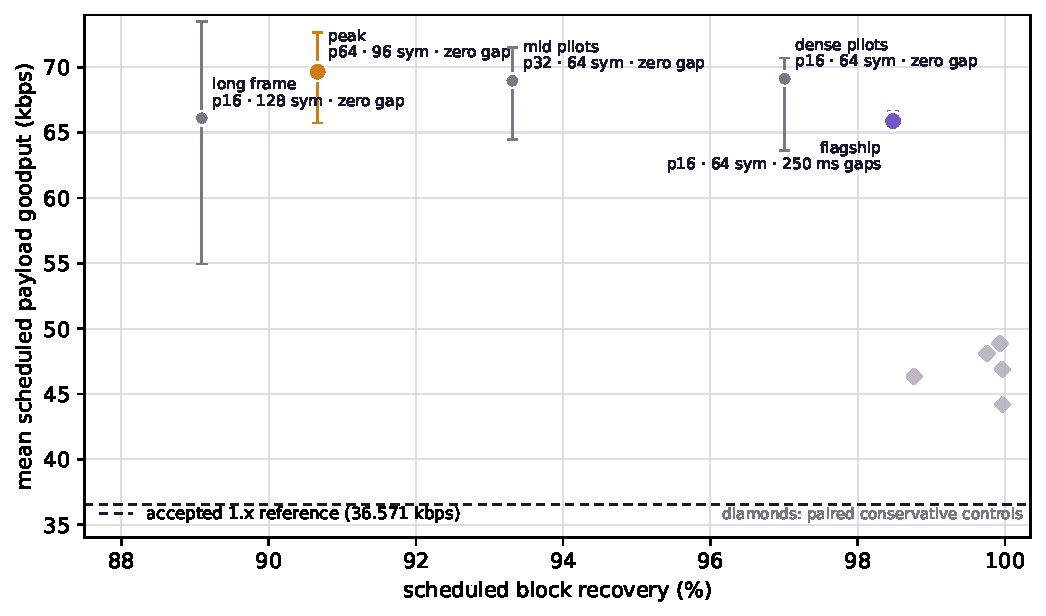
\includegraphics[width=0.98\linewidth]{cyrinx2-goodput-reliability.pdf}
\caption{Observed goodput--recovery trade space from five separate complete
campaigns. Circles are candidates, diamonds their paired controls, and
vertical whiskers are observed per-run ranges. The sessions were not a
randomized pilot/frame-length factorial; no causal trend line is implied.}
\label{fig:frontier}
\end{figure}

\section{Same-capture receiver comparison}
\label{sec:replay}

The fresh flagship captures were replayed through two frozen decoders with
identical capture identity, timing, decode margins, payloads, and automatic
diversity policy. The only receiver-family difference was global-only versus
pilot-local reliability. The legacy receiver recovered 3,868/4,280 blocks
(90.374\%); the current receiver recovered 4,215/4,280 (98.481\%). The +347
blocks are an 8.108-percentage-point gain, and reduce failed blocks from 412
to 65. All eight runs improved and none regressed.

\begin{figure}[ht]
\centering
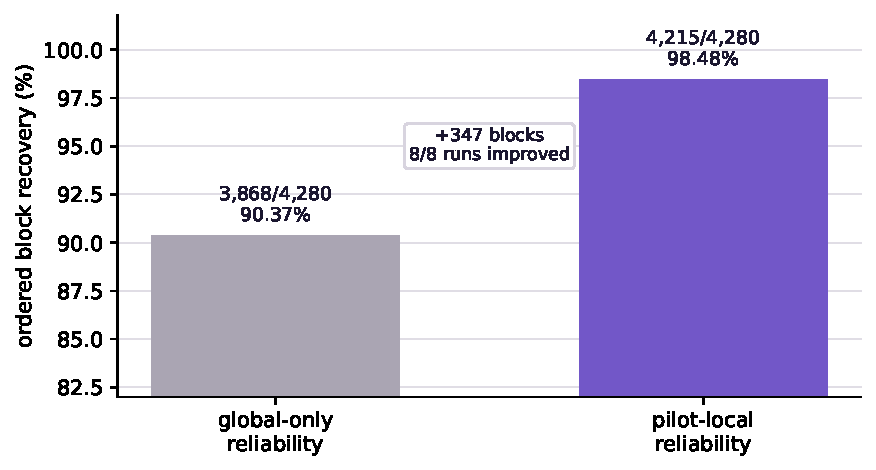
\includegraphics[width=0.82\linewidth]{cyrinx2-receiver-replay.pdf}
\caption{Aggregate same-capture receiver replay. The retained PCM and slot
timing are identical; only global-only versus pilot-local reliability changes.
This isolates the estimator as a bundle, not its boxcar, interpolation, edge,
or 25/75-blend subcomponents.}
\label{fig:replay}
\end{figure}

Because all other profile changes are held fixed in this replay, it is the
strongest causal evidence in the 2.0 campaign. It does not isolate microphone
selection, which is the same on both sides, and it does not show that the
specific smoothing width or blend is optimal.

\section{Separate zero-gap frontier}
\label{sec:frontier}

Removing the four 250\,ms gaps changes the schedule and denominator class. It
is useful for studying continuous streaming but cannot replace the
schedule-comparable flagship. The highest eight-pair mean used CP96, pilot
spacing 64, 64-QAM rate 2/3, and 96 data symbols: 69.652\,kb/s scheduled
(65.731--72.641), 68.636\,kb/s gross, and 6,129/6,760 recovered blocks
(90.666\%). Its control achieved 48.103\,kb/s and 4,509/4,520 blocks
(99.757\%). It won 8/8 pairs and failed the reliability gate.

\begin{table}[ht]
\centering
\caption{Cross-session observed frontier. All candidates used CP96 and
64-QAM rate 2/3. Values are descriptive rather than a randomized factorial.}
\label{tab:frontier}
\small
\begin{tabular}{lrrrr}
\toprule
Pilots / symbols / gap & Mean kb/s & Range kb/s & Blocks & Recovery \\
\midrule
16 / 64 / 250\,ms & 65.875 & 65.266--66.641 & 4,215/4,280 & 98.481\% \\
16 / 64 / zero & 69.110 & 63.650--70.708 & 4,152/4,280 & 97.009\% \\
32 / 64 / zero & 68.960 & 64.449--71.507 & 4,143/4,440 & 93.311\% \\
64 / 96 / zero & \textbf{69.652} & 65.731--72.641 & 6,129/6,760 & 90.666\% \\
16 / 128 / zero & 66.102 & 54.938--73.504 & 7,662/8,600 & 89.093\% \\
\bottomrule
\end{tabular}
\end{table}

The observations do not show a monotonic amortization win. The denser p16
64-symbol zero-gap profile gave nearly the peak mean with materially higher
recovery. The 128-symbol run was slower and less reliable than the shorter
zero-gap alternatives. Since configurations were run in separate sessions,
these differences may mix pilot density, frame length, channel drift, HVAC,
and other temporal variation.

\section{Setbacks and rejected branches}
\label{sec:setbacks}

Optimization was dominated by branches that appeared plausible in rate
arithmetic and failed over the air. Table~\ref{tab:negative} retains the
failures so that the 65.875\,kb/s result is not mistaken for a monotonic sweep
to a predetermined answer.

\begin{longtable}{p{0.20\linewidth}p{0.29\linewidth}p{0.43\linewidth}}
\caption{Negative and inconclusive Cyrinx 2.0 experiments.}\label{tab:negative}\\
\toprule
Branch & Measurement & Interpretation \\
\midrule
\endfirsthead
\toprule
Branch & Measurement & Interpretation \\
\midrule
\endhead
CP48 & Candidate-first screen: 93/107, 63.277\,kb/s. Opposite order:
64/107, 43.546\,kb/s. Both CP240 controls: 75/75. & The apparently fast first
screen was order-sensitive; CP48 was not promoted. \\
\addlinespace
64-QAM rate 3/4 & 87/121 blocks, 57.925\,kb/s, versus 75/75 control. & More
code rate did not produce usable net goodput at this constellation density. \\
\addlinespace
64-QAM rate 5/6 & 24/134 at volume 50 (15.979\,kb/s); 21/134 at volume 60
(13.982\,kb/s). & Weaker FEC failed, and more level did not rescue it. \\
\addlinespace
Lower edge 600\,Hz & 60/110, 39.948\,kb/s, versus 77/77 control. & Stopped at
the predeclared gate. With no reverse order or same-MCS 1.1\,kHz control, this
rejects promotion but does not isolate the lower edge causally. \\
\addlinespace
Volume 70 & Higher capture peak without clipping; only 24/75 and 57/75 versus
near-error-free volume-50 qualification. & Endpoint level is not a monotonic
proxy for post-DSP demodulation quality. \\
\addlinespace
128 symbols & 66.102\,kb/s and 7,662/8,600 (89.093\%). & Longer frames did not
amortize their way to a better result in this session. \\
\addlinespace
Fixed-comb channel tracking & Frequency-local changes remain interpolated
between repeatedly observed pilot bins. & A decision-directed update at
$\alpha=0.05$ may propagate wrong 64-QAM decisions; it remains unvalidated and
unshipped. \\
\addlinespace
Both speakers, same waveform & Historical left+right playback in this geometry
raised EVM from about 0.06 (left only) to about 0.5. & Blind summation is not
MIMO. The second speaker needs orthogonal sounding and precoding/spatial
multiplexing, not duplication. \\
\bottomrule
\end{longtable}

The results also corrected an earlier over-broad statement that uniform
64-QAM ``does not close.'' High-rate 64-QAM r3/4 failed in the earlier cell;
64-QAM r2/3 closes with the current CP, pilot lattice, local reliability, and
qualified route. A modulation name without code rate, CP, pilots, receiver,
and cell is not a portable claim.

\section{Calibration and device policy lessons}
\label{sec:calibration}

The research harness now constructs a deterministic tone matrix: the Mac left
speaker is exercised while both Android input channels are retained, a safety
gate is evaluated, and then the right speaker is exercised. Ramped single
tones from 997\,Hz through 21.001\,kHz and two intermodulation pairs measure the
end-to-end speaker--room--microphone--OS path. Sync markers estimate clock and
alignment; the plan binds the target, route, calibration artifact, and exact
waveform hashes. This is relative channel characterization, not an SPL meter,
and two logical channels alone do not prove independent capsules.

The current physical runner measures the two Mac outputs against the two
Android inputs. A complete product calibration should generalize this to every
available transmitter/receiver pair, including each device's own speaker-to-
microphone paths where simultaneous platform routing permits it. That
same-device matrix is a design requirement, not a completed 2.0 feature.

Orientation is useful context but not a sufficient Android source policy. A
face-down accelerometer state suggests that a rear-facing capsule may be
exposed, but OEM routing can map \texttt{CAMCORDER}, \texttt{UNPROCESSED},
\texttt{MIC}, stereo masks, and sample rates differently. Cyrinx therefore
binds an observed route signature and tone response. On this face-up Pixel,
48\,kHz stereo \texttt{UNPROCESSED} exposed direct bottom and back channels;
selecting \texttt{CAMCORDER} merely from pose would have discarded measured
evidence. A future policy can use accelerometer pose as a prior, then confirm
the actual route with a short tone check.

\section{Ultrasonic and pleasant-audible modes}
\label{sec:ultrasonic}

The companion research record demonstrates a one-way ultrasonic profile, not
an integrated 2.0 mode. At 96\,kHz, the Mac-to-Pixel route carried about
9\,kb/s in 18.5--23.9\,kHz using 16-QAM rate 3/4 with 39/39 blocks recovered.
The reverse coherent route did not close: Pixel and iPhone micro-speakers
radiated high-frequency power but exhibited large phase jitter above about
18\,kHz. Figure~\ref{fig:ultrasonic} shows the retained iPhone repetitions.

\begin{figure}[ht]
\centering
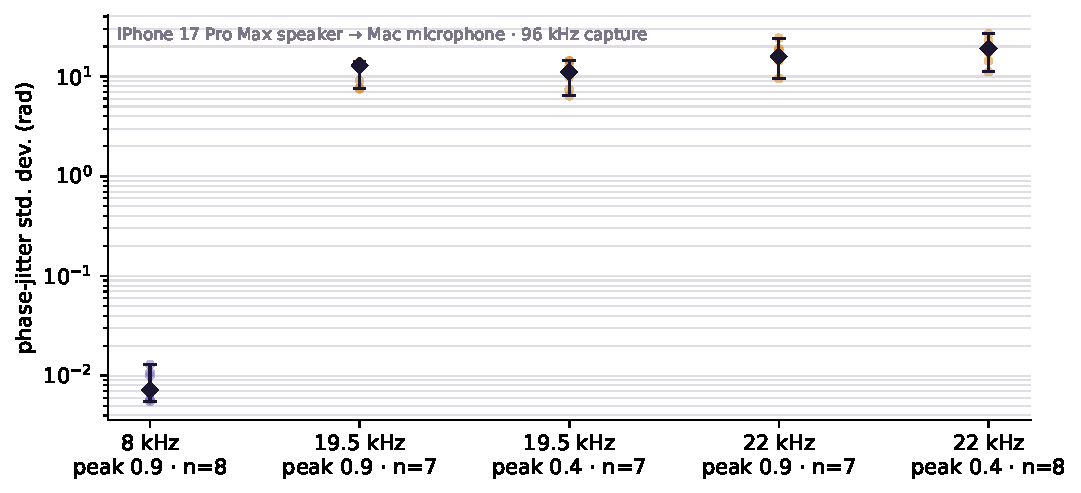
\includegraphics[width=0.96\linewidth]{cyrinx2-ultrasonic-phase.pdf}
\caption{Detrended phase jitter for the iPhone 17 Pro Max speaker measured by
the Mac microphone at 96\,kHz. Points are 7--8 retained valid repetitions per
condition; diamonds and whiskers show median and observed range. High-frequency
power is present, but the phase coherence needed by QAM is not.}
\label{fig:ultrasonic}
\end{figure}

An integrated ultrasonic mode therefore needs a C profile, 96\,kHz route and
capability negotiation, device-specific characterization, and a non-coherent
phone-uplink fallback such as energy-detected MFSK or OOK. The likely symmetric
rate is much lower than the audible downlink because the mobile transmit
transducer, not the nominal bandwidth, is limiting.

A ``pleasant audible'' mode has not been implemented or listening-tested.
The credible research direction is perceptual spectral shaping rather than a
claim that ordinary OFDM static can simply be made quiet: measure room tone,
reserve frequencies near masking energy, window transitions, avoid chirp-like
onsets, constrain crest factor, and optimize a lower-rate waveform under a
declared listening protocol. Candidate approaches include sparse/staggered
tones, shaped spread spectrum, or perceptually weighted OFDM. The objective
must include listener ratings and acoustic level, not goodput alone.

\section{Implementation convergence}
\label{sec:implementation}

The portable C codec is the canonical PHY implementation. It owns modulation,
FEC, demodulation, MRC, automatic receiver selection, and pilot-local
reliability. Swift is a thin binding and retains deterministic contract tests.
Python remains valuable as an independently implemented research oracle and
campaign referee. The Android Kotlin demodulator is still a legacy fork;
the Pixel 2.0 campaign captured PCM on Android and decoded it with frozen C on
the host rather than through an Android JNI binding.

This four-language state is a real drift risk. The convergence plan is not to
rewrite the same DSP four times: bind Android to the C core through JNI, keep
Swift thin, retain Python only where independence improves verification, and
run every binding against the same receiver-contract and captured-waveform
fixtures before retiring Kotlin DSP. Until then, \cyrtwo{} is not a real-time
mobile transport mode.

\section{Threats to validity and next experiments}
\label{sec:limits}

The strongest claim is narrow by design. It covers one Mac, one Pixel, one
near-field pose, one Android route, one speaker channel, and a short campaign
on one day. HVAC cycled, room tone and SPL were uninstrumented, and the phone
was unusually close to the laptop speaker. The result is downlink-only. It
does not include app/ADB setup, a preceding sounder, ARQ, retransmission
latency, or application framing. Host-side batch decoding does not establish
real-time CPU, buffering, or on-device behavior. Eight pairs support the exact
within-session sign test but not broad device or room generalization.

Multiple development screens preceded the fresh confirmatory campaign. The
prospective pair design protects the final comparison, but the selected
profile is still the product of exploratory work in this cell. The raw
evidence is locally retained but not yet in a public archival bundle. Finally,
the automatic selector's 26/14 decisions prove payload-independent operation,
not that the selector is optimal.

The next research sequence is:
\begin{enumerate}
  \item qualify reliability first: replicate across days, HVAC states, levels,
        small offsets, and held-out devices; optimize an explicit goodput--loss
        objective rather than the mean alone;
  \item run a randomized pilot-spacing/frame-length factorial, including
        staggered known pilots and a code rate near 0.70;
  \item integrate the C receiver on Android, measure real-time end-to-end
        transport with block ARQ, and include sounding/cold-start overhead;
  \item execute the separately labeled fixed 3-foot campaign, remeasuring
        route, room tone, level, and delay spread rather than inheriting the
        near-field profile;
  \item test orthogonal two-speaker sounding and a true 2$\times$2 channel
        matrix before attempting precoding or spatial multiplexing; and
  \item evaluate ultrasonic and pleasant-audible modes under per-device
        calibration and, for pleasant audio, a preregistered listening metric.
\end{enumerate}

\section{Conclusion}

\cyrtwo{} raises the measured Mac-to-Pixel mean from the accepted
36.571\,kb/s schedule target to 65.875\,kb/s, and from its prospective paired
control's 44.199\,kb/s by 49.0\%. The gain comes from shorter guards, lower
pilot overhead, 64-QAM with stronger rate-2/3 coding, a qualified route,
frequency-local known-pilot reliability, and payload-independent use of two
microphones. Same-capture replay attributes +347 recovered blocks to the local
reliability receiver as a bundle. The candidate's 98.481\% recovery remains
below the control's 99.967\%, and the faster 69.652\,kb/s zero-gap class falls
to 90.666\%. The engineering conclusion is therefore not that near-field
acoustic goodput has been maximized; it is that materially higher measured
goodput is available, while reliability-qualified generalization is now the
limiting problem.

\appendix
\section{Evidence bindings and availability}
\label{sec:evidence}

The tracked aggregate source is the repository's
\href{https://github.com/dweekly/cyrinx/blob/main/scratch/hw20k/evidence/pixel7a-cyrinx2-2026-07-17/results-ledger.json}{Pixel results ledger}.
The tracked
\href{https://github.com/dweekly/cyrinx/tree/main/scratch/hw20k/evidence/pixel7a-faceup-volume50-v1}{route-qualification bundle}
retains target, route, and level provenance. The manuscript figures are
generated by \texttt{gen-cyrinx2-paper-figures.py} from that ledger and the
tracked iPhone phase-coherence JSON.

\begin{longtable}{p{0.25\linewidth}p{0.66\linewidth}}
\caption{Content bindings for the two primary campaigns.}\label{tab:hashes}\\
\toprule
Artifact & SHA-256 \\
\midrule
\endfirsthead
\toprule
Artifact & SHA-256 \\
\midrule
\endhead
Flagship plan &
\hash{fe295a7835061ccb55f9ffe277c455c}{97b3487decb6e9da38b01af61c32e05ef} \\
Flagship completed manifest &
\hash{3d46bf7eccf669a6d29ca6593662c6c4}{23710c24062aebe6c9ec16ddf7646ec6} \\
Flagship frozen decoder &
\hash{bd7e52acaf1d9c7a1994d5a350af8ba}{f2ea2fef03f47ed3a0f59fd8513c0327c} \\
Same-capture replay file &
\hash{57522f6b3cafb5e925a2bfbb1ea70e54}{48999a17052aa3201a6f4f91367009bc} \\
Same-capture canonical content &
\hash{e25d099550d4e72b9686a6bf5a3c54e}{c6b7b75b5eb52aa761bca42994e12a50b} \\
Zero-gap plan &
\hash{8e5f1062dcccc42bbfac866a8659bf8d}{1884dd54bb054a9f42d944a1919e966b} \\
Zero-gap completed manifest &
\hash{9846a33717c18e457169578217dbbdabe}{740eaa26c09965cb24ce128c9d1e462} \\
Zero-gap frozen decoder &
\hash{c6e4e5adc0865a379dc036c549cef4cd}{91528152ffffa66ee2fdf9be47580956} \\
Route signature, canonical JSON &
\hash{8da17a36acdd7a79d0f70f9fc085b99}{a8faf508f862387edec3b093180a827d0} \\
Calibration qualification &
\hash{ec28faa1b67bfcea8a615ee4b6dd6d85}{f3427d79fae075e30b5b6ffd84ff165d} \\
Target provenance &
\hash{5f87abe17227315ae77ea3632bdd21cbf}{e3364ae5875b1f7d35ca2a04a0c8251} \\
\bottomrule
\end{longtable}

The ledgers and qualification records are public in the source tree. Full
manifests, raw captures, frozen binaries, and detailed replay reports are
currently ignored local artifacts. A stable supplemental archive is required
before describing the experiment as publicly reproducible from raw PCM.

\end{document}
